\chapter{Evaluation}\label{ch:evaluation}

\section{Reference Implementation}

A reference implementation of \cref{sec:asynchronous} is available on GitHub\footnote{\url{https://github.com/cwru-xlab/sharetrace-akka}}. Actors are implemented using the Akka toolkit\footnote{\url{https://doc.akka.io/docs/akka/2.8.5/typed/index.html}}, which offers high performance for large-scale actor systems. Experimental results indicate that the reference implementation can process contact networks with at least 1 million individuals and 10 million contacts on a single machine, so it is suitable for small-scale and medium-scale experiments. In addition to using the Akka toolkit, several other optimizations are implemented.
\begin{itemize}
  \item To reduce the size of event logs and result files, individual actor identifiers follow zero-based numbering and event records are serialized using the Ion format\footnote{\url{https://amazon-ion.github.io/ion-docs}} with shortened field names.
  \item To reduce memory usage, FastUtil\footnote{\url{https://fastutil.di.unimi.it}} data structures are used, including a specialized integer-based JGraphT\footnote{\url{https://jgrapht.org}} graph implementation \citep{Michail2020}. Also, singletons \citep{Gamma1995}, primitive data types, and reference equality are preferred where feasible and do not impact readability.
  \item To reduce runtime and increase throughput, logging is performed asynchronously with Logback\footnote{\url{https://logback.qos.ch/index.html}} and the LMAX Disruptor\footnote{\url{https://lmax-exchange.github.io/disruptor}}.
\end{itemize}

\Cref{fig:arrow-diagram} shows the dependencies among the application components. Contextualizing this implementation with prior implementations of the driver-monitor-worker (DMW) framework (see \cref{sec:dmw-framework}), \class{RiskPropagation} is the driver, \class{Monitor} is the monitor, and \class{User} is the worker. The key difference between this implementation and previous implementations of the DMW framework is that workers are stateful, which is necessary for decentralization.
\begin{figure}[htbp]
\begin{equation*}
  \class{Main} \rightarrow \class{Runner} \rightarrow \class{RiskPropagation} \rightarrow \class{Monitor} \rightarrow \class{User} \rightarrow \class{Contact}
\end{equation*}
\caption[Arrow diagram of the reference implementation]{Arrow diagram of the reference implementation.}
\label{fig:arrow-diagram}
\end{figure}

\Cref{sec:asynchronous} describes the behavior of a \class{User} and \class{Contact}. In order to evaluate \class{RiskPropagation}, each \class{User} logs the following types of \class{UserEvent}:
\begin{itemize}
  \item \class{ContactEvent}: logged when the \class{User} receives an unexpired \class{ContactMessage}; contains the \class{User} identifier, the \class{Contact} identifier, and the contact time.
  \item \class{ReceiveEvent}: logged when the \class{User} receives an unexpired \class{RiskScoreMessage}; contains the \class{User} identifier, the \class{Contact} identifier, and the \class{RiskScoreMessage}.
  \item \class{UpdateEvent}: logged when the \class{User} updates its exposure score; contains the \class{User} identifier, the previous \class{RiskScoreMessage}, and the current \class{RiskScoreMessage}.
  \item \class{LastEvent}: logged when the \class{User} receives a \class{PostStop} Akka signal\footnote{\url{https://doc.akka.io/docs/akka/current/typed/actor-lifecycle.html\#stopping-actors}} after the \class{Monitor} has stopped; contains the \class{User} identifier and the time of logging the last event, besides \class{LastEvent}; used to detect the end time of message passing.
\end{itemize}
For reachability analysis, a \class{RiskScoreMessage} contains the identifier of the \class{User} that propagated it and the identifier of the \class{User} that first sent it.

The \class{Monitor} is an actor that is responsible for transforming the \class{ContactNetwork} into a collection of \class{User}s and terminating when no \class{UpdateEvent} has occurred for a period of time. The \class{Monitor} logs several types of \class{LifecycleEvent}, ordered according to when they are logged during execution:

\begin{multicols}{2}
\begin{enumerate}
  \item \class{RiskPropagationStart}
  \item \class{CreateUsersStart}
  \item \class{CreateUsersEnd}
  \item \class{SendContactsStart}
  \item \class{SendContactsEnd}
  \item \class{SendRiskScoresStart}
  \item \class{SendRiskScoresEnd}
  \item \class{RiskPropagationEnd}
\end{enumerate}
\end{multicols}

\class{RiskPropagation} logs execution properties, creates an Akka \class{ActorSystem} that creates a \class{Monitor} actor and sends it a \class{RunMessage}, and then waits until the \class{ActorSystem} terminates. Each execution of \class{RiskPropagation} is associated with a unique key that is included in each event record as mapped diagnostic context (MDC)\footnote{\url{https://logback.qos.ch/manual/mdc.html}}.

The \class{Runner} specifies how \class{RiskPropagation} is created and invoked, usually through some combination of statically defined behavior and runtime configuration.

Finally, \class{Main} is the entry point into the application. It is responsible for parsing \class{Context}, \class{Parameters}, and \class{Runner} from configuration and invoking \class{Runner} with \class{Context} and \class{Parameters} as inputs. \class{Context} makes application-wide information accessible, such as the system time and user time\footnote{System time is always the wall-clock time and is included in each logged event record. User time is configurable to either be the wall-clock time or fixed at the reference time. The latter ensures that no \class{RiskScoreMessage} or \class{ContactMessage} expires across executions of \class{RiskPropagation}.}, a pseudorandom number generator, \class{Runner} configuration, and loggers. \class{Parameters}, as the name suggests, is a collection of parameters that modify the behavior of the \class{Monitor}, \class{User}s, and \class{Contact}s.

To analyze the logs that are generated during the execution of \class{RiskPropagation}, they are transformed into a tabular dataset as follows:
\begin{enumerate}
  \item Load the execution properties for all executions of \class{RiskPropagation} that are associated with the same configuration.
  \item Process the stream of event records with one \class{EventHandler} per execution of \class{RiskPropagation}.
  \item Collect the results from each \class{EventHandler} and store them in a file.
  \item To analyze different configurations of \class{RiskPropagation}, load multiple result files and augment the results of each \class{RiskPropagation} execution with its execution properties.
  \item Flatten the resulting data structure and store the tabular dataset.
\end{enumerate}

For evaluation, the following event handlers were implemented:

\begin{itemize}
  \item \class{Reachability}: aggregates \class{ReceiveEvent}s that involve a distinct sender and receiver to determine the influence set cardinality, source set cardinality, and message reachability of each \class{User}.
  \item \class{Runtimes}: aggregates \class{LifecycleEvent}s and \class{LastEvent}s to determine the runtime of creating \class{User}s, sending \class{ContactMessage}s, sending \class{RiskScoreMessage}s, message passing, and the overall execution of \class{RiskPropagation}. Message-passing runtime is the time elapsed from the start of sending \class{RiskScoreMessage}s until the last \class{LastEvent}.
  \item \class{UserEventCounts}: aggregates \class{UserEvent}s to determine the frequency of each subtype for each \class{User}.
  \item \class{UserUpdates}: aggregates \class{UpdateEvent}s to determine the new exposure score of each \class{User} and the change in value.
\end{itemize}

\section{Experimental Design}

The following experiments were used to evaluate \class{RiskPropagation}.
\begin{enumerate}[ref={Experiment \arabic*}]
  \item How do the send coefficient and tolerance affect accuracy and efficiency?\label{item:parameters}
  \item Do the distributions of risk scores and contact times affect runtime?\label{item:distributions}
  \item How does the contact network topology affect runtime?\label{item:topology}
\end{enumerate}

\labelcref{item:parameters} was completed first to determine suitable parameter values for the remaining experiments. \labelcref{item:distributions} was conducted before \labelcref{item:topology} to determine the necessity of evaluating all combinations of data distributions. That is, if the type of data distribution was found to have a statistically nonsignificant effect on the runtime of \class{RiskPropagation}, then the complexity of \labelcref{item:topology} could be meaningfully reduced. While \labelcref{item:distributions} and \labelcref{item:topology} focus on benchmarking the reference implementation, more advanced simulation-based analysis of ShareTrace with COVI-AgentSim \citep{Gupta2020} is the subject of future work.

All experiments utilized the same random graphs: Barabasi-Albert graphs \citep{Barabasi1999}, Erd\"{o}s-R\'{e}nyi $G_{n,m}$ graphs \citep{Erdos1959}, Watts-Strogatz graphs \citep{Watts1998}, and random regular graphs \citep{Kim2003}. These graphs were selected because they exhibit, to varying extents, aspects of real-world complex networks \citep{Newman2003}, such as contact networks; they are available in the JGraphT library; and they all are parametric, either directly or indirectly, in the size and order of the network. The last property allowed the effects of the topology to be isolated.

The following describes the parametrization of each type of contact network. Barabasi-Albert graphs are parametrized by the order $n$, the initial order $n_0$, and the increase in size $m_0$ upon each incremental increase in order. The latter two parameters are determined by solving \cref{eq:Barabasi-Albert-optimization}, where $\fracpart(x)$ is the fractional part of a real number $x$.
\begin{argmini}{n_0, m_0}{\fracpart(m_0)}{\protect\label{eq:Barabasi-Albert-optimization}}{}
  \addConstraint{n_0}{\in \intInterval{1}{n - 1}}
  \addConstraint{m_0}{\in \intInterval{1}{n_0}}
  \addConstraint{m_0}{= \frac{2m - n_0 (n_0 - 1)}{2(n - n_0)}}
\end{argmini}
Erd\"{o}s-R\'{e}nyi graphs are parametrized by the order $n$ and the size $m$. Random regular graphs are parametrized by the order $n$ and, using the degree sum formula, the degree $d = \lfloor 2m / n \rfloor$. Lastly, Watts-Strogatz graphs \citep{Watts1998} are parametrized by the order $n$, the rewiring probability $p$, and the number of nearest neighbors $k = d + (d \bmod 2)$, which must be even.

\Cref{tab:default-parameters} specifies the default parameter values and seed for pseudorandom number generation. \Cref{tab:experiments} specifies the experiment configurations. All experiments used fixed user time. The following sampling process was used to generate risk scores and contact times.  Given the probability density function $f_X$ and the cumulative distribution function $F_X$ of a random variable $X$, sample a value $x \sim f_X$ and evaluate $c \cdot F_X(x)$ for some scalar $c \in \reals$. Risk scores are composite data types, so risk score values and risk score times were sampled independently. Because risk scores are probabilities, $c = 1$ was used to scale the values. When sampling the times of risk scores and contacts, $c = \pScoreExpiry$ and $c = \pContactExpiry$ were used, respectively.

\begin{table}[htbp]
  \centering
  \begin{tabular}{ll}
    \toprule
    Parameter & Default value \\
    \midrule
    Transmission rate, $\pTransmissionRate$ & \num{0.8}\\
    Send coefficient, $\pSendCoefficient$ & \num{1}\\
    Tolerance, $\pTolerance$ & \num{0}\\
    Time buffer, $\pTimeBuffer$ & \qty{2}{days}\\
    Risk score expiry, $\pScoreExpiry$ & \qty{14}{days}\\
    Contact expiry, $\pContactExpiry$ & \qty{14}{days}\\
    Flush timeout & \qty{3}{seconds}\\
    Idle timeout & \qty{1}{minute}\\
    Seed & \num{12345}\\
    \bottomrule
  \end{tabular}
  \caption[Default parameter values for experiments]{Default parameter values for experiments.}
  \label{tab:default-parameters}
\end{table}

\begin{sidewaystable}[htbp]
  \centering
  \renewcommand{\arraystretch}{2}
  \begin{tabular}{lccc}
    \toprule
    Aspect & \labelcref{item:parameters} & \labelcref{item:distributions} & \labelcref{item:topology} \\
    \midrule
    Order $n$ and size $m$ & $\begin{aligned} n &= 10^4 \\ m &= 5 \cdot 10^4 \end{aligned}$ & $\begin{aligned} n &= 10^4 \\ m &= 5 \cdot 10^4 \end{aligned}$ & $\begin{matrix} n \in \setBuilder{10^5x}{x \in \intInterval{1}{10}} \\ \times \\ m \in \setBuilder{10^6x}{x \in \intInterval{1}{10}} \end{matrix}$ \\
    \hline
    Parameters & $\begin{matrix} \pSendCoefficient \in \setBuilder{10^{-1}x}{x \in \intInterval{8}{20}} \\ \pTolerance \in \setBuilder{10^{-3}x}{x \in \intInterval{1}{10}} \end{matrix}$ & Defaults & Defaults \\
    \hline
    Distributions & $\{\text{Uniform}, \text{Standard normal}\}^3$ & $\{\text{Uniform}, \text{Standard normal}\}^3$ & Uniform \\
    \hline
    Repetitions & 5 & 1 burn-in + 5 & 1 burn-in + 5 \\
    \hline
    Networks evaluated & 160 (40 per type) per parameter & 160 (40 per type) & 400 (100 per type) \\
    \bottomrule
  \end{tabular}
  \caption[Experiment configurations]{Experiment configurations. See \cref{tab:default-parameters} for default parameter values. In \labelcref{item:parameters}, the send coefficient and tolerance were evaluated independently. The notation $X^k$ is used to denote the $k$-ary Cartesian power of the set $X$. A ``burn-in'' repetition was used for \labelcref{item:distributions} and \labelcref{item:topology} to avoid measuring the impact of Java class loading.}
  \label{tab:experiments}
\end{sidewaystable}

\section{Results}

\subsection{\labelcref{item:parameters}}

\begin{figure}[htbp]
  \centering
  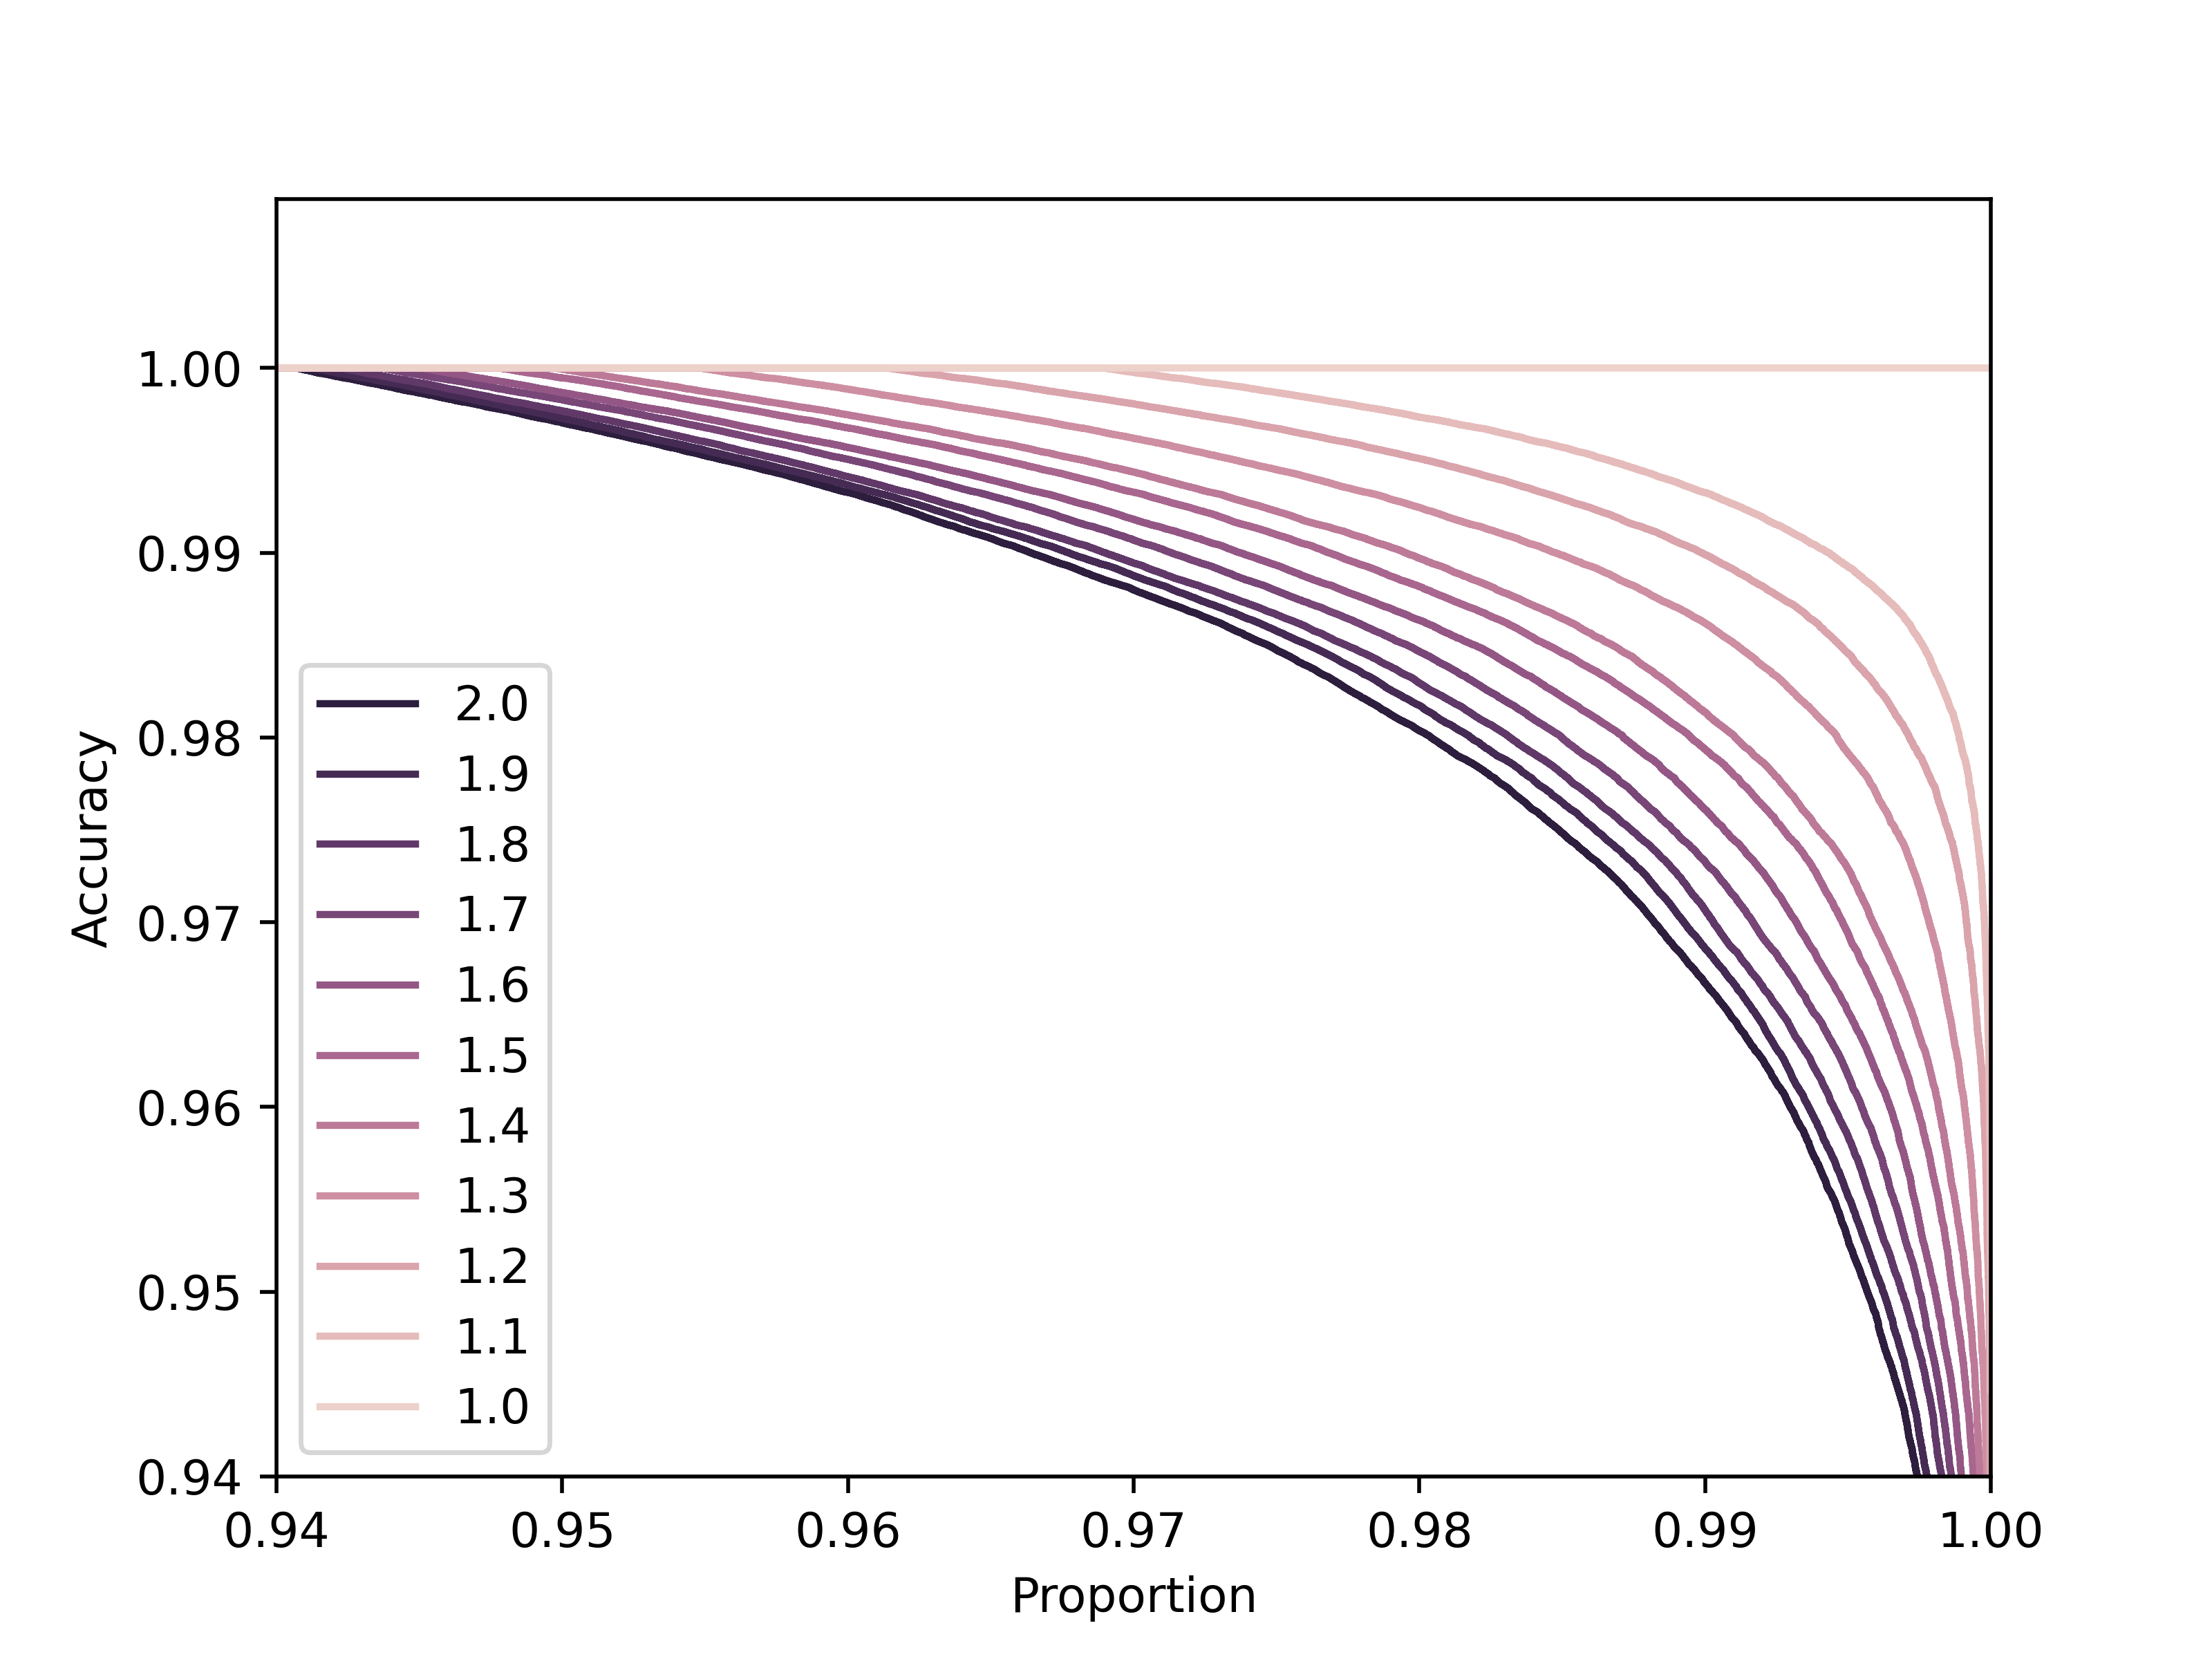
\includegraphics[width=\textwidth]{accuracy-send-coefficient}
\end{figure}

\begin{sidewaystable}[htbp]
\centering
\begin{tabular}{
  S
  S[table-auto-round, table-format = 1.3]
  S[table-auto-round, table-format = 1.3]
  S[table-auto-round, table-format = 1.3]
  S[table-auto-round, table-format = 1.3]
  S[table-auto-round, table-format = 1.3]
  S[table-auto-round, table-format = 1.3]
  S[table-auto-round, table-format = 1.3]
  S[table-auto-round, table-format = 1.3]
  S[table-auto-round, table-format = 1.3]
}
\toprule
& \multicolumn{9}{c}{Percentile} \\
\cmidrule{2-10}
{Send coefficient} & {0} & {0.01} & {0.1} & {1} & {2} & {3} & {4} & {5} & {6} \\
\midrule
1.0 & 1.0 & 1.0 & 1.0 & 1.0 & 1.0 & 1.0 & 1.0 & 1.0 & 1.0 \\
1.1 & 0.945 & 0.965 & 0.979 & 0.993 & 0.997 & 1.0 & 1.0 & 1.0 & 1.0 \\
1.2 & 0.916 & 0.952 & 0.972 & 0.99 & 0.995 & 0.998 & 1.0 & 1.0 & 1.0 \\
1.3 & 0.883 & 0.937 & 0.961 & 0.986 & 0.992 & 0.996 & 0.999 & 1.0 & 1.0 \\
1.4 & 0.882 & 0.922 & 0.952 & 0.981 & 0.99 & 0.994 & 0.997 & 1.0 & 1.0 \\
1.5 & 0.86 & 0.911 & 0.947 & 0.979 & 0.988 & 0.993 & 0.997 & 0.999 & 1.0 \\
1.6 & 0.855 & 0.9 & 0.94 & 0.976 & 0.986 & 0.992 & 0.996 & 0.999 & 1.0 \\
1.7 & 0.848 & 0.891 & 0.934 & 0.973 & 0.985 & 0.991 & 0.995 & 0.998 & 1.0 \\
1.8 & 0.84 & 0.884 & 0.93 & 0.971 & 0.983 & 0.989 & 0.994 & 0.998 & 1.0 \\
1.9 & 0.826 & 0.879 & 0.924 & 0.969 & 0.982 & 0.989 & 0.994 & 0.997 & 1.0 \\
2.0 & 0.817 & 0.871 & 0.92 & 0.967 & 0.98 & 0.988 & 0.993 & 0.997 & 1.0 \\ 
\bottomrule
\end{tabular}
\caption[Aggregate accuracy percentiles]{Aggregate accuracy percentiles}
\label{tab:accuracy-aggregate}
\end{sidewaystable}

\begin{table}[htbp]
\centering
\begin{tabular}{SSS[table-auto-round, table-format = 1.3]}
\toprule
{Send coefficient} & {Frequency} & {Proportion} \\ 
\midrule
1.0 & 11258 & 1.0 \\
1.1 & 2899 & 0.981 \\
1.2 & 2622 & 0.976 \\
1.3 & 2535 & 0.972 \\
1.4 & 2465 & 0.967 \\
1.5 & 2622 & 0.963 \\
1.6 & 2392 & 0.959 \\
1.7 & 2329 & 0.955 \\
1.8 & 2856 & 0.951 \\
1.9 & 3144 & 0.946 \\
2.0 & 556924 & 0.941 \\ 
\bottomrule
\end{tabular}
\caption[Aggregate accuracy frequency]{Aggregate accuracy frequency}
\label{tab:accuracy-aggregate-frequency}
\end{table}

\clearpage

\subsection{\labelcref{item:distributions}}

A one-way analysis of variance (ANOVA) was considered for determining if the mean message-passing runtimes associated with different data distributions are statistically different. ANOVA assumes the observations are independently sampled, normally distributed, and homoscedastic within groups. The message-passing runtimes were indeed independently sampled. To test the latter two assumptions, the Shapiro-Wilk test \cite{Shapiro1965} and the Fligner-Killeen test \cite{Fligner1976} were applied, respectively. While the runtimes were found to be homoscedastic ($p > \num{0.05}$), they were not normally distributed ($p < \num{0.05}$). As such, the Kruskal-Wallis test was applied instead of a one-way ANOVA, which indicated there is insufficient evidence to reject the null hypothesis that the median message-passing runtimes are statistically different across data distributions. See \cref{tab:runtime-hypothesis-tests} for the test statistics and associated $p$-values. Note, this experiment assumes this statistical significance holds for other data distributions and network topologies.

\begin{sidewaystable}[htbp]
\centering
\begin{tabular}{lSSSSSS}
  \toprule
  & \multicolumn{2}{c}{Shapiro-Wilk test} & \multicolumn{2}{c}{Fligner-Killeen test} & \multicolumn{2}{c}{Kruskal-Wallis test} \\
  \cmidrule(lr){2-3} \cmidrule(lr){4-5} \cmidrule(lr){6-7}
  Network type & {Statistic} & {$p$-value} & {Statistic} & {$p$-value} & {Statistic} & {$p$-value} \\
  \midrule
  All & 0.672 & 2e-17 & 2.256 & 0.944 & 7.030 & 0.426 \\
  Barabasi-Albert & 0.646 & 1e-8 & 4.535 & 0.716 & 5.241 & 0.631 \\
  Erd\"{o}s-R\'{e}nyi & 0.472 & 8e-11 & 4.865 & 0.676 & 3.231 & 0.863 \\
  Random regular & 0.583 & 2e-9 & 3.900 & 0.791 & 3.022 & 0.883 \\
  Watts-Strogatz & 0.437 & 3e-11 & 2.474 & 0.929 & 5.971 & 0.543 \\
  \bottomrule
\end{tabular}
\caption[Runtime hypothesis tests]{Runtime hypothesis tests.}
\label{tab:runtime-hypothesis-tests}
\end{sidewaystable}